\documentclass[tikz,border=3.14mm]{standalone}
\usepackage{tkz-euclide}
\usetikzlibrary{backgrounds}

\begin{document}

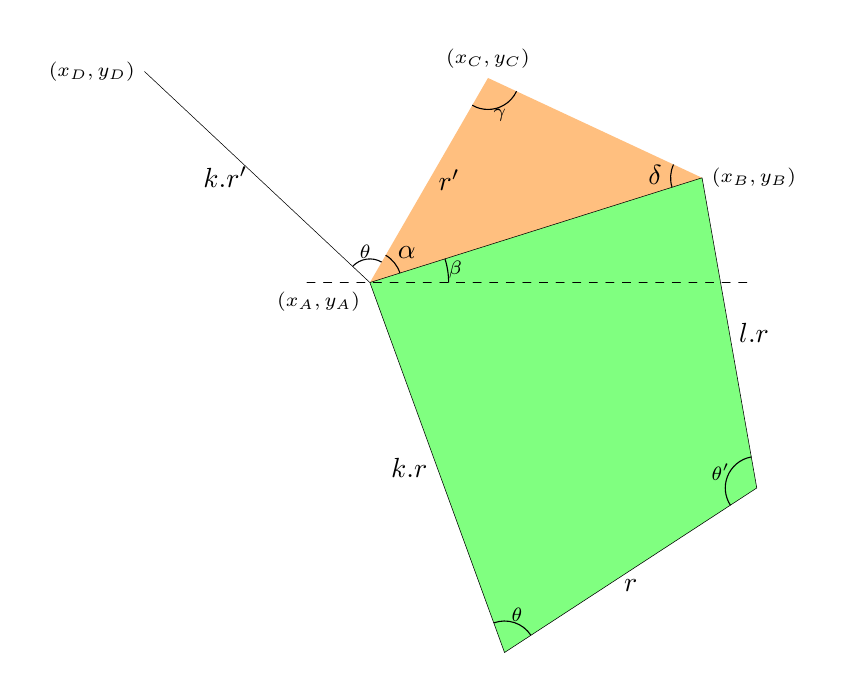
\begin{tikzpicture}[background rectangle/.style={fill=white!45}, show background rectangle]
  \tkzInit
  % Defining the triangle
  \tkzDefPoint(0,0){C}
  \tkzDefShiftPoint[C](-120:3){A}
  \tkzDefShiftPoint[C](-25:3){B}
  \tkzDefShiftPoint[A](4,0){O}
  \tkzDefShiftPoint[A](-70:5){H}
  \tkzDefShiftPoint[B](-80:4){I}

  \tkzCalcLength(A,B)\tkzGetLength{dAB}
  \tkzCalcLength(A,H)\tkzGetLength{dAH}
  \tkzCalcLength(A,C)\tkzGetLength{dAC}
  \tkzCalcLength(H,I)\tkzGetLength{dHI}
  \pgfmathsetmacro\k{\dAH/\dHI}
  % Theta
  \tkzFindAngle(I,H,A)\tkzGetAngle{angtheta}
  % Theta'
  \tkzFindAngle(B,I,H)\tkzGetAngle{angthetap}
  % Beta + alpha, (angle between AC and the horizontal line
  \tkzFindAngle(O,A,C)\tkzGetAngle{alphabeta}
  
  \tkzDefShiftPoint[A]({\angtheta+\alphabeta}:{\dAC*\k}){D}
  \tkzDrawSegment(A,D)
  % \tkzFillPolygon[fill = red!50 ](A,C,E,D)
  % \tkzFillPolygon[fill = blue!50 ](C,B,G,F)
  \tkzFillPolygon[fill = green!50](B,A,H,I)
  \tkzFillPolygon[fill = orange,opacity=.5](A,B,C)
  % \tkzDrawPolygon[line width = 1pt](A,B,C)
  % \tkzDrawPolygon[line width = 1pt](A,C,E,D)
  % \tkzDrawPolygon[line width = 1pt](C,B,G,F)
  \tkzDrawPolygon(B,A,H,I)
  % Labels
  % Points
  \tkzLabelPoint[below left](A){\scriptsize $(x_A, y_A)$}
  \tkzLabelPoint[right](B){\scriptsize $(x_B, y_B)$}
  \tkzLabelPoint[above](C){\scriptsize $(x_C, y_C)$}
  \tkzLabelPoint[left](D){\scriptsize $(x_D, y_D)$}
  % \tkzLabelPoint[above](E){\scriptsize $(x_E, y_E)$}
  % \tkzLabelPoint[above](F){\scriptsize $(x_F, y_F)$}
  % \tkzLabelPoint[right](G){\scriptsize $(x_G, y_G)$}
  % Segments
  % \tkzLabelSegment[below](A,B){}
  \tkzLabelSegment[right](A,C){$r'$}
  \tkzLabelSegment[below](H,I){$r$}
  \tkzLabelSegment[left](A,H){$k.r$}
  \tkzLabelSegment[right](I,B){$l.r$}
  \tkzLabelSegment[left](A,D){$k.r'$}
  % Horizontal line through A
  \tkzDefLine(A,O)
  \tkzDrawLine[dashed](A,O)
  % Marking angles
  % First internal angle
  \tkzMarkAngle[size=.4](I,H,A)
  \tkzLabelAngle[pos=.5](I,H,A){\scriptsize $\theta$}
  % First internal angle in new square
  \tkzMarkAngle[size=.3](C,A,D)
  \tkzLabelAngle[pos=.4](C,A,D){\scriptsize $\theta$}
  % Second internal angle
  \tkzMarkAngle[size=.4](B,I,H)
  \tkzLabelAngle[pos=.5](B,I,H){\scriptsize $\theta'$}
  
  \tkzMarkAngle[size=.4](A,C,B)
  \tkzLabelAngle[pos=.5](A,C,B){\scriptsize $\gamma$}
  % Angle BAC
  \tkzMarkAngle[size=.4](B,A,C)
  \tkzLabelAngle[pos=.6](B,A,C){$\alpha$}
  % Angle ABC
  \tkzMarkAngle[size=.4](C,B,A)
  \tkzLabelAngle[pos=.6](C,B,A){$\delta$}
  % Phase of AC
  \tkzMarkAngle[size=1](O,A,B)
  \tkzLabelAngle[pos=1.1](O,A,B){\scriptsize $\beta$}

\end{tikzpicture}
\end{document}


%%% Local Variables:
%%% mode: latex
%%% TeX-master: "figure3"
%%% End:
